\documentclass[10pt,twocolumn]{report}

\usepackage{ulem}

% -------------------- Document Layout --------------------

\usepackage{geometry}        % For page layout
\geometry{
    a4paper,                 % Paper size
    margin=0.5in,            % General margin
    top=1in,                 % Top margin
    bottom=1in,              % Bottom margin
    left=0.6in,              % Left margin
    right=0.6in              % Right margin
}

% -------------------- Header and Footer Setup --------------------

\usepackage{fancyhdr}        % For custom headers and footers
\usepackage{xcolor}          % For text color customization

\pagestyle{fancy}            % Set fancy header/footer style
\renewcommand{\headrulewidth}{0.4pt}   % Header rule thickness
\renewcommand{\footrulewidth}{0.4pt}   % Footer rule thickness
\setlength{\headheight}{15pt} % Header height (adjust as needed)

% Define custom color
\definecolor{lightgray}{gray}{0.7}

% Clear existing header and footer settings
\fancyhf{}

% Set up the left, center, and right parts of the header
\lhead{\textcolor{lightgray}{\small Jason Joel Pinto}} % Left header
\chead{}                                        % Center header (empty)
\rhead{\hfill \textcolor{lightgray}{\small Early Prediction and Progression Modelling of Alzheimer’s Disease}} % Right-aligned header

% Set up the left, center, and right parts of the footer
\lfoot{\textcolor{lightgray}{\small Gisma University of Applied Sciences}}  % Left footer
\cfoot{\textcolor{lightgray}{\large \bfseries \thepage}}                   % Center footer (page number)
\rfoot{\hfill \textcolor{lightgray}{\small December, 2024}}                % Right footer with date

\renewcommand{\headrulewidth}{0.4pt}
\renewcommand{\footrulewidth}{0.4pt}
\setlength{\headheight}{10pt}
\renewcommand{\headrule}{\textcolor{lightgray}{\rule{\textwidth}{0.3pt}}}
\renewcommand{\footrule}{\textcolor{lightgray}{\rule{\textwidth}{0.3pt}}}

% -------------------- Font and Text Customization --------------------

\usepackage[utf8]{inputenc}  % UTF-8 encoding
\usepackage[T1]{fontenc}     % Font encoding
\usepackage{ebgaramond}      % Use EB Garamond font
\usepackage{caption}         % For customizing captions

% Set caption style to small and italic
\captionsetup{font={small,it} }  % small font and italic style for captions

% -------------------- Line Spacing --------------------

\usepackage{setspace}        % For line spacing
\onehalfspacing              % Set line spacing to 1.5

% -------------------- Title and Section Formatting --------------------

\usepackage{titlesec}        % For title formatting
\titleformat{\title}[block]
  {\normalfont\bfseries\Huge}{\thetitle}{0pt}{}  % Title formatting (Huge font size, bold)

\titleformat{\chapter}[block]
  {\normalfont\bfseries\LARGE}{}{0pt}{\Large}     % Chapter headings (LARGE font size, bold)
  
\titleformat{\section}
  {\normalfont\Large\bfseries}{\thesection}{1em}{}  % Section headings (Large font size, bold)

\titleformat{\subsection}
  {\normalfont\normalsize\bfseries}{\thesubsection}{1em}{}  % Subsection headings (normal size, bold)

\titlespacing*{\chapter}{0pt}{-10pt}{15pt}   % Adjust chapter spacing

% -------------------- Page Break Management --------------------

% Remove page breaks between chapters
\newcommand{\chapterbreak}{\vspace{1.5cm}} % Adjust spacing if needed
\titleclass{\chapter}{straight}[\chapterbreak] 

% -------------------- Bibliography and Citations --------------------

\usepackage[backend=biber]{biblatex}  % For bibliography management
\addbibresource{mybib.bib}            % Add .bib file for references

% -------------------- Hyperlinks --------------------

\usepackage{hyperref}        % For clickable links
\hypersetup{
    colorlinks=true,
    linkcolor=blue,
    urlcolor=blue,
    citecolor=blue
}

% -------------------- Images and Captions --------------------

\usepackage{graphicx}        % For including images
\usepackage{caption}         % For customizing captions
\usepackage{enumitem}        % For customizations like "nosep"


% Begin document
\begin{document}

% Title page
%\begin{titlepage}
%    \centering
%    {\bfseries\Huge Early Prediction and Progression Modelling of Alzheimer’s Disease Using Multi-Modal Time Series Data \par} % Title (22pt, bold)
%    \vspace{1.5cm}
%    {\Large Jason Joel Pinto \par} % Author name (14pt)
%    \vfill
%    A Thesis Submitted in Partial Fulfillment of the Requirements for the Degree of \par
%    {\large MSc in Data Science, AI and Digital Marketing \par} % Program (12pt)
%    \vspace{1cm}
%    {\large Gisma University of Applied Sciences \par} % University (12pt)
%    {\large Dec, 2024 \par} % Month and year (12pt)
%    \vfill
%\end{titlepage}

\begin{titlepage}
    \begin{center}
        % University Logo (Optional)
        % \includegraphics[width=0.15\textwidth]{university_logo.png} \\[1cm]
        
        % University Name
        \textsc{\Large Gisma University of Applied Sciences} \\[1.5cm]
        \vfill  
        % Title
        % \rule{\linewidth}{0.2mm} \\[0.4cm]
        {\bfseries\Huge Early Prediction and Progression Modelling of Alzheimer’s Disease \\[0.4cm]
        Using Multi-Modal Data} \\[0.4cm]
        % \rule{\linewidth}{0.2mm} \\[1.5cm]
        \vfill        
        % Author Name
        {\Large \textbf{Jason Joel Pinto}} \\[2cm]
        \vfill
        % Submission Text
        {\large A Thesis Submitted in Partial Fulfillment of the Requirements for the Degree of} \\[0.5cm]
        {\Large MSc in Data Science, AI and Digital Marketing} \\[1.5cm]
        
        % Date
        {\large December, 2024}
        
        \vfill
    \end{center}
\end{titlepage}

% Abstract
\chapter*{Abstract}
\addcontentsline{toc}{chapter}{Abstract}

Alzheimer's is a neurological disorder, which is a main cause for dementia \cite{Ewers2011}. There are a lot of researches are that being conducted right now all over the world for the Alzheimer disease. A disease such as alzheimer's is very hard to predict as studies show that it can be cause due to multiple factors. Now when it comes to Multi modal machine learning models, it integrates different data sources such as a persons demographic data, lifestyle, medical history, clinical assessment, and cognitive assessment etc. This has sparked a new idea to process the data and understand a patter to detect the disease at a early stage. To achieve this various advanced machine learning models are being used.

As new advancement are being done in the medical fields, the aged population is going to rise. And more and more people, their relatives and family members are going to face deadly diseases such as Alzheimer's. Studies has shown that the early detection of alzheimer's Disease is more likely to get treated or leads to less serious problems when compared to the medications started at a later stage \cite{Cummings2024}.

For this study the data being used is based on the Alzheimer's research organization called Open Access Series of Imaging Studies (OSIS). Various traditional as well and deep learning models are used to find the best model as well as the best parameters in order to reach a most accuracy score possible. The measurement scores used to select the best model out of all will be Recall, Accuracy, F1-score and Precision. 

Incomplete.... Need to fill the rest.


% Acknowledgments
% \chapter*{Acknowledgments}
% \addcontentsline{toc}{chapter}{Acknowledgments}
% Write your acknowledgments here.

% Table of contents
\tableofcontents
\listoffigures % Optional
\listoftables  % Optional

% Chapters
\chapter{Introduction}

Alzheimer's is a neurological problem that starts with a build up of proteins called amyloid plaques and neurofibrillary tangles. This leads to the brain cells to die over time and this leads to the shrinkage of the brain size\cite{mayo_alzheimers_2024}. Studies show us that about 5.4 million people in the States have Alzheimer's. And the studies show upward trend in the newer generations in getting Alzheimer's Disease. It is expected to increase by 10 million people. As of today every 68 second and new person is being diagnosed by Alzheimer's Disease. And the studies show that by 2050 this is going to decrease to 33 seconds\cite{2012131}. Between the year 2000 and 2017 the deaths reported due to alzheimer's have been increased by 143 \%\cite{2019321}. Alzheimer's is a disease which get's worse over the years, it keeps on progressing and the worst thing it is not reversible. Once worsened a lot of time and efforts go into the alzheimer's diseace. Which might end up being one of the costliest disease for any countries economy\cite{10.3389/fnagi.2024.1363458}. Hence it becomes very important that it is diagnosed as a early stage so that it can be controlled and treated. If it is detected early then doctor's with the help of medications can make sure that brain damage is not worsened. Currently magnetic resonance imaging (MRI),functional magetic resonance imaging(fMRI), computer tomography and positron emission tomography (PET) are used in order to early detect the Alzheimer's disease. These technologies are very expensive, very time consuming task and not very accessible for everyone as it Requirement sophisticated machines.

Machine Learning can be used to find if there is a way where one can find if there is a way models can find patterns which makes it possible to detect the disease at even earlier stage. As there are various studies that are being conducted all around the world, there are various data that are available which can be used by the machine learning models to analyze and early detect the disease. Based on prior researches, the researchers have numerical data's related to a persons MRI's and biomarkers in a persons body. With help of these they find whether a person is demented or not. If these data are used and ML model be developed which will be able to predict the will be lead to inexpensive diagnosis and can be made easily available to more and more people. In addition to that the automated model will be more accurate and also removes all human errors. 

\begin{figure}[h!]
    \centering
    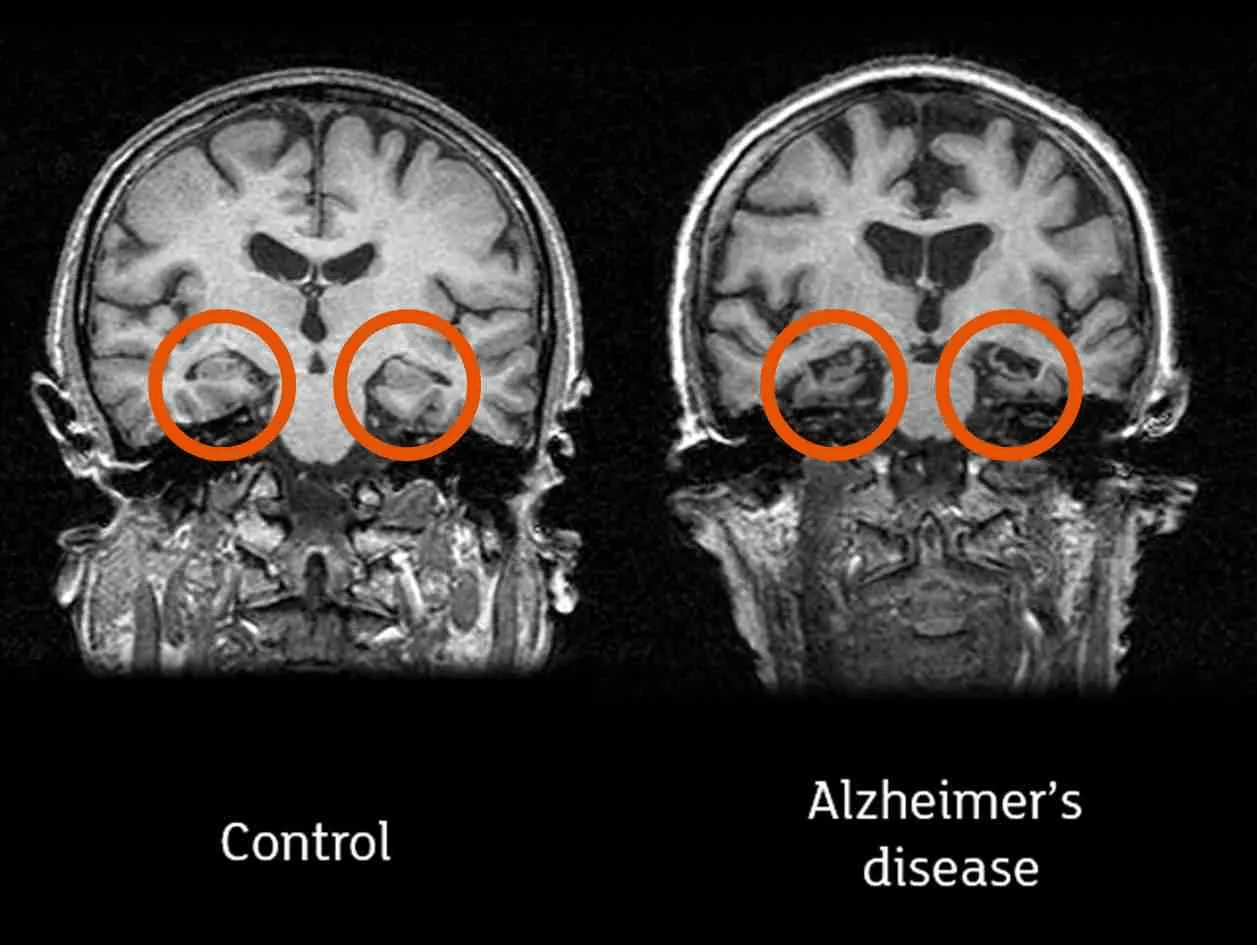
\includegraphics[width=0.8\columnwidth]{figures/fig1.png}  % Adjust the width to your liking
    \caption{Comparison of a normal brain (left) and an Alzheimer's patient's brain (right).\\Images credit: Professor John O'Brien, University of Cambridge and Newcastle University} % Caption for the image
    \label{fig:alzheimers_brain} % Label to reference the image later in the document
\end{figure}

A person with Alzheimer's disease will not be aware that he might be having a disease can ultimately lead to be a very dangerous disease. This is because the symptoms of Alzheimer's are very hard to find. It can be different to different people. The person can still do all the regular chores he does day to day without any problems. Having said that there will be some problems he might be facing while doing these activities, like for example not able to remember words, or not remembering names etc. People around him will definitely notice that this person has trouble remembering stuff. This is the reason why doctor as a first step usually conducts a medical interview where the person will be asked some questions. With the help of this he will be able to get a ball park idea whether he might have Alzheimer's or not. Some of the symptoms of Alzheimer's as follows,
\begin{enumerate}[nosep]
    \item Forgetting things, misplacing things, and missing meetings.
    \item Forgetting names and events.
    \item Not able to recall incidents happened in the past.
    \item Problems with audio visual memory.
    \item Being absent minded.
    \item Agitation and restlessness
\end{enumerate}

The symptoms of Alzheimer's becomes more evident when the disease progresses and one grows old. The person starts notices that the symptoms that he previously had are slowly slowly getting worse and worse. At later stages of AD it becomes very difficult to even communicate with the person as he does not remember anything. He forgets to even do the basic things that he has been taught to do since his childhood. This the stage when they will need continuous Assistance. 

\chapter{Motivation}

\begin{figure}[h!]
    \centering
    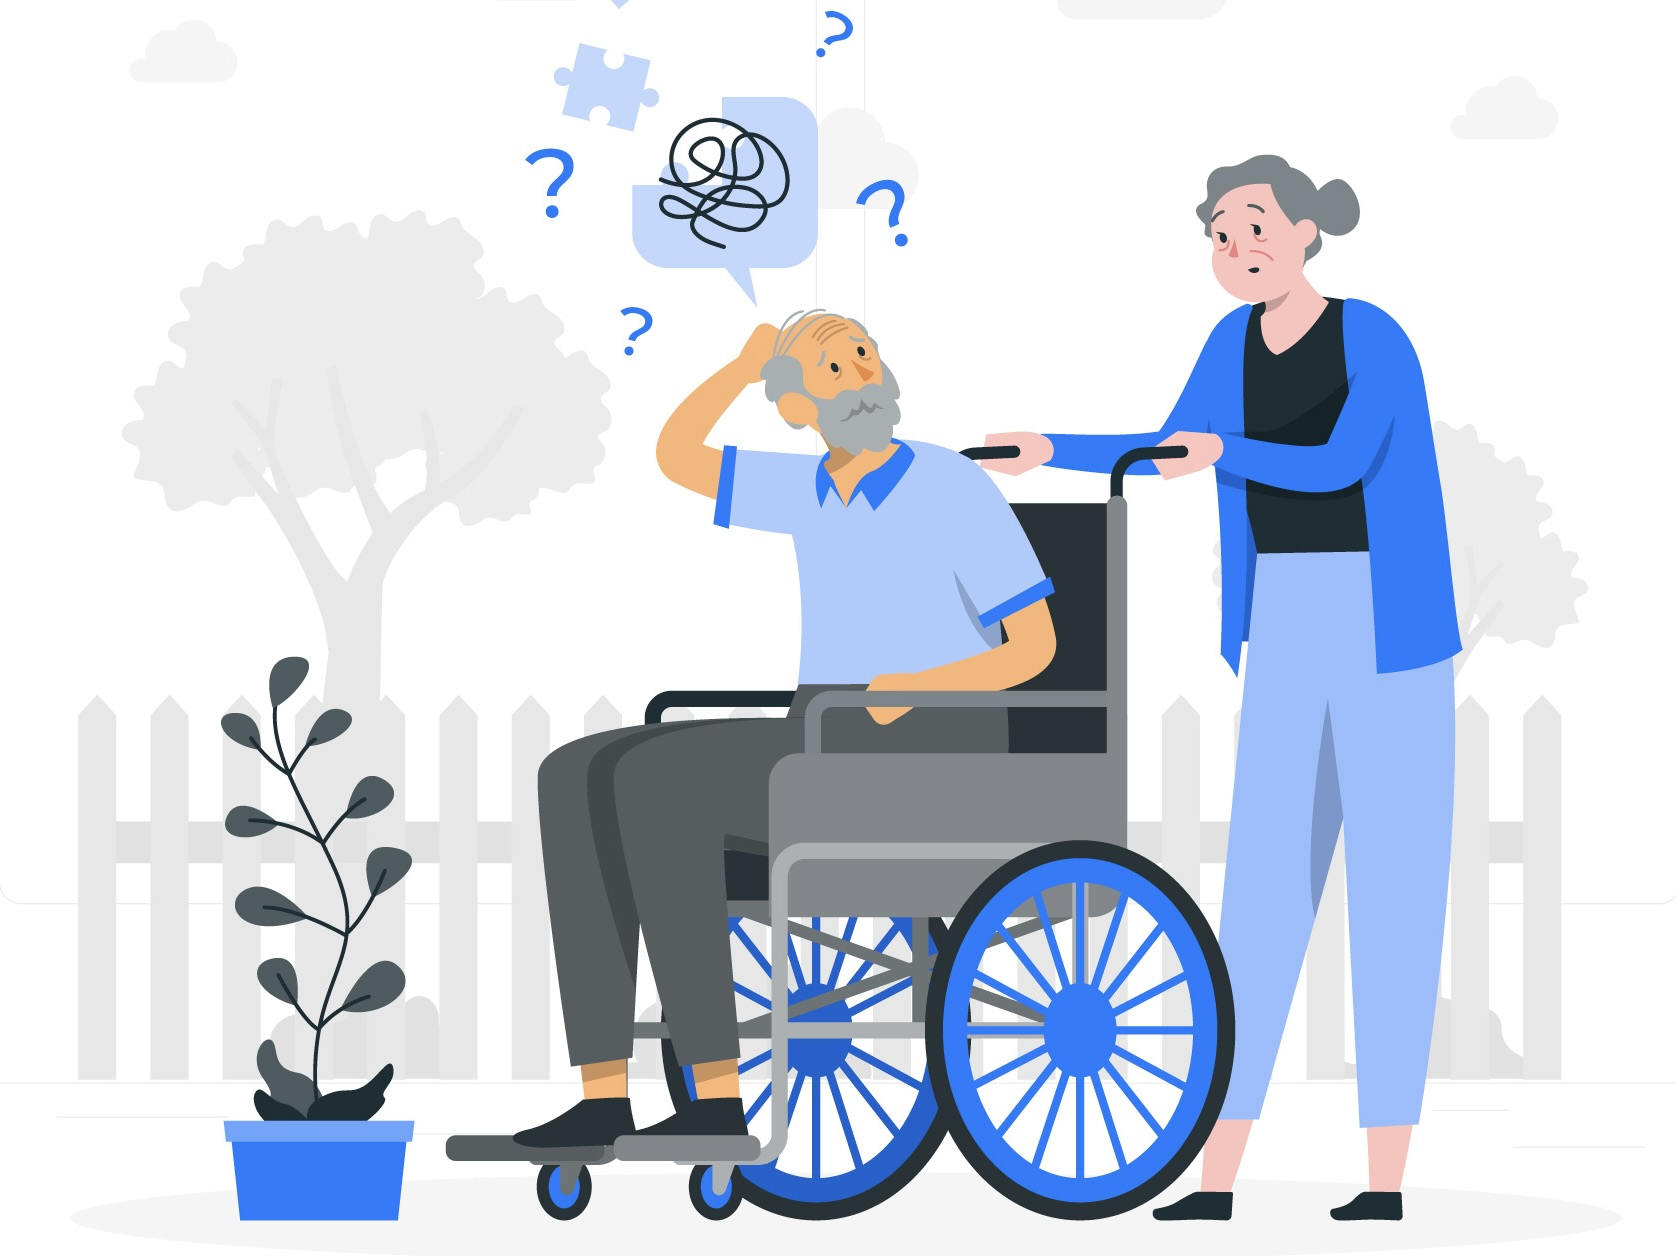
\includegraphics[width=0.8\columnwidth]{figures/fig2.jpeg}  % Adjust the width to your liking
    \caption{Person suffering from Dementia} % Caption for the image
    \label{fig:alzheimers_patient} % Label to reference the image later in the document
\end{figure}

Alzheimer's is considered as one of the most challenging disease in the modern medicine research. And this disease not only effects the individual but also impacts the people around him/her that is family, doctors and also the hospitals. As the people effected by this disease are increase at a rapid rate around us, there is a need to develop a better way to diagnose and prevent this disease. Particularly, there is a high demand for a system that will detect the disease at a early stage. So that the medical team can stop the disease from getting worse at the old age which might cause a big economic burger for the patients.

The motivation to write this thesis came from the fact that there are sophisticated diagnostics options available at the moment which are very expensive, time-consuming and they are not accessible for of people. But the main problem is even after spending a lot of money on these diagnostic procedures, it cannot detect it at a very earlier stage. Doctors use MRI's and PET scans which are very accurate but they machines used for this are very special and needs an expert to use them. Additionally, even after analyzing a persons brain in these scans, the disease is not detected at a early stage because the small changes that are happening in the brain are very different to find when compared to the normal aging of a persons brain. 

With the advanced Machine Learning techniques we can try to fix these problems that are currently there. By using the datasets that available online the advanced Machine Learning models can find patterns in the datasets which is hard to find using a naked human eyes. This will help in detecting the  Alzheimer's disease at a very earlier stage. 

Personally for me this paper is driven by the fact that I have seen many people around me struggling with Alzheimer's disease in their old age. I have seen it first hand how much time, money and effort does it take for their family to take care of them in that situation. As it is a disease that gradually gets worse, they slowly start losing their memory and identity. Having witnessed this I have seen how much effort goes into taking care of a Alzheimer's patient. This has motivated me to provide my Contribution to this communicate and make a difference. Hence, my aim in this research is to create a model will be able to predict the possibility of the disease at a earlier stage. 


\chapter{Contribution}

The contribution of this thesis paper is to use the advanced Machine Learning algorithms to find a solution to problems of early detection of the Alzheimer's disease. This will include implementing various different advance machine learning models to improve the predicting of the disease based on the MRI images that we are using for this research. The main contributions are such as:

\begin{enumerate}[nosep]
    \item \textbf{Develop a Machine Learning Model to predict the disease at a Early Stage:} In this research patient's MRI images will be analyzed which are divided into various stages of Alzheimer's and build a Classification Model using these images. This will enable to find a pattern even at a early stage of Alzheimer's find it.

    \sout{ \textbf{Evaluation of Machine Learning and Deep Learning Models:} Multiple traditional and state-of-the-art deep learning models were implemented and compared, including random forests, support vector machines (SVM), and neural networks. The performance of these models was rigorously evaluated using metrics like accuracy, precision, recall, and F1-score to identify the most effective prediction approach.}

    \sout{ \textbf{Parameter Optimization for Enhanced Accuracy:} A detailed hyperparameter tuning process was undertaken to optimize model performance. Techniques such as grid search and cross-validation were employed to ensure the robustness and generalizability of the selected models.}

    \sout{ \textbf{Utilization of Publicly Available Datasets:} The study extensively utilized data from the Open Access Series of Imaging Studies (OASIS), a recognized resource in Alzheimer’s research. This ensured the research adhered to ethical guidelines while leveraging high-quality, real-world data.}

    \sout{ \textbf{Early Detection Potential with Cost-Effective Solutions:} By focusing on machine learning approaches, the research aims to provide scalable and cost-effective solutions for early AD diagnosis. This could significantly improve accessibility, especially in resource-constrained settings where sophisticated imaging technologies are not viable.}

    \sout{ \textbf{Contributions to Medical AI Research:} Beyond practical applications, this study contributes to the broader field of medical AI by exploring the interpretability of predictive models. Attention was given to ensuring that model predictions align with known clinical findings, thereby increasing trust in machine learning applications for healthcare.}

    \sout{ \textbf{Open-Source Codebase and Documentation:} To facilitate future research, the methodologies, datasets, and source code have been documented comprehensively. The study encourages replication and extension of the findings by other researchers in the domain.}

\end{enumerate}

These contributions underscore the potential of advanced AI techniques in transforming Alzheimer’s Disease diagnosis, offering hope for timely interventions and improved patient outcomes.

\chapter{Related Work}
Your introduction goes here.

\chapter{Literature Review}
Your literature review goes here.

\chapter{Methodology}
Your methodology goes here.

\chapter{Results}
Your results go here.

\chapter{Discussion}
Your discussion goes here. 123456

\chapter{Conclusion}
Your conclusion goes here.

% Appendices
\appendix
\chapter{Appendix Title}
Appendix content goes here.

% References
\cleardoublepage
\printbibliography
\end{document}
